\chapter[Revisão Estruturada da Literatura]{Revisão Estruturada da Literatura}

Neste capítulo descrevem-se, os procedimentos adotados 
para identificar, selecionar, avaliar e sintetizar a literatura relevante ao tema deste trabalho. 
A estratégia de busca concentrou-se na base Scopus, escolhida por sua ampla cobertura de 
periódicos e conferências de referência nas áreas de Computação e Engenharia de Software, 
bem como por seus recursos de filtragem e exportação de metadados que facilitam a rastreabilidade 
do processo \cite{Scopus2025}. 

\section{Protocolo}

O protocolo da revisão estruturada da literatura utilizado foi inspirado nas diretrizes propostas por 
\citeonline{kitchenham2007guidelines}, com o objetivo de assegurar transparência e reprodutibilidade do processo.

\subsection{String de busca}

Para estruturar a string de busca, adotamos o protocolo PICO (Patient, Intervention, Comparison, Outcome), 
originalmente proposto para área da saúde. O protocolo precisou ser adaptado para o contexto da Engenharia de Software \cite{pai_clinical_2004}.
Como apresentado na Figura \ref{fig:pico}, o protocolo pode ser representado em forma de diagrama de Venn para facilitar a 
visualização das relações entre os elementos.

\begin{figure}[H]
    \centering
	\caption{Representação protocolo PICO}
    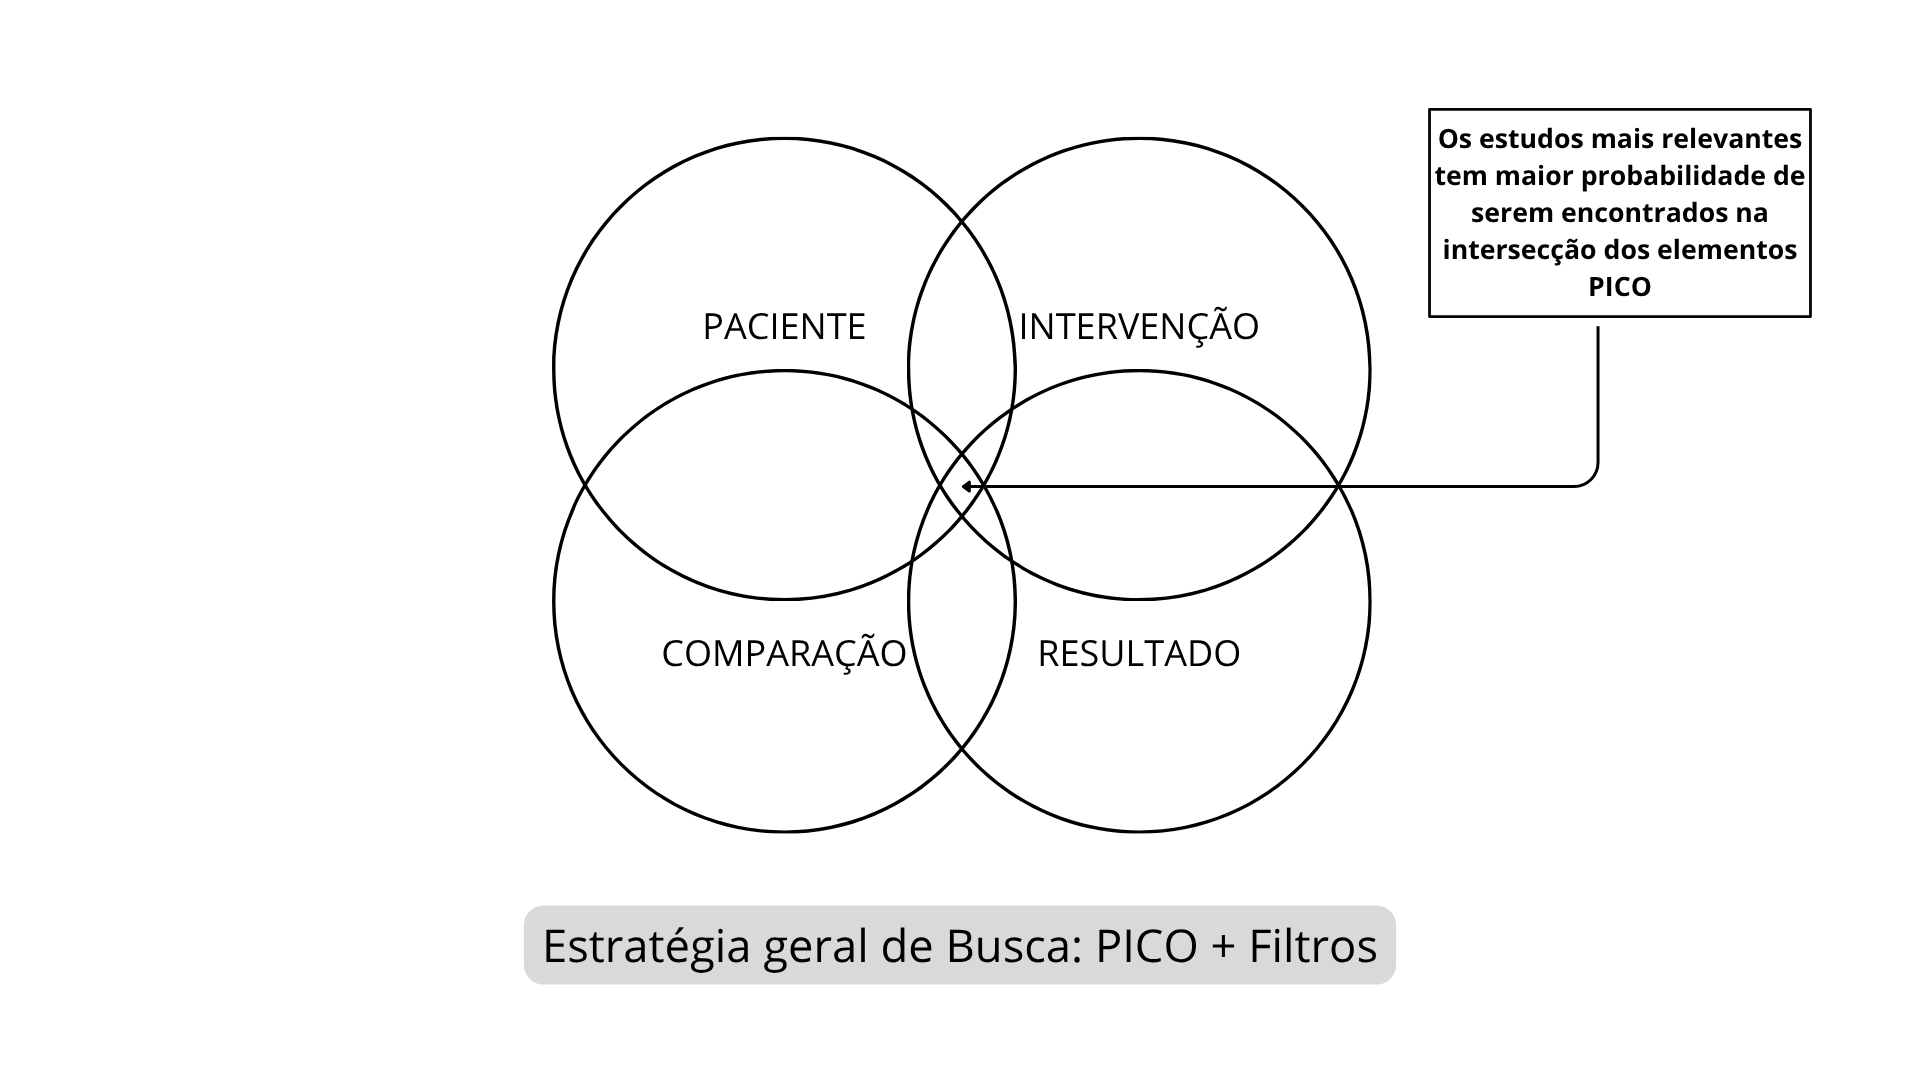
\includegraphics[width=1\textwidth]{figuras/venn-PICO.png}

    \label{fig:pico}
	Fonte: Adaptado de \citeonline{pai_clinical_2004}
\end{figure}

Considerando o PICO no contexto da Engenharia de Software, cada elemento assume um significado 
próprio. O termo \textit{Paciente} (Population), originalmente associado ao perfil clínico, 
passa a denotar a área específica da engenharia de software. A \textit{Intervenção} (Intervention), antes entendida como tratamento, corresponde 
aqui às abordagens avaliadas, tais como metodologias, métodos, técnicas, ferramentas ou procedimentos de 
desenvolvimento e análise. Os \textit{Resultados} (Outcomes) preservam sua essência, representando os efeitos 
observados e as métricas de interesse. Já a \textit{Comparação} (Comparison), por se alinhar mais diretamente 
à área médica, pode não ser aplicável a todos os estudos em Engenharia de Software. As definições 
utilizadas neste trabalho encontram-se na Tabela \ref{tab:picoadaptado}.

\begin{table}[H]
    \centering
	\caption{PICO Adaptado}
    \begin{tabular}{|p{4cm}|p{3cm}|p{5cm}|}
        \hline
        \textbf{Elementos} & \textbf{Palavra chave} & \textbf{Sinônimos e Termos Relacionados} \\
        \hline
        \textbf{População} & Software engineering & software development, software system, software application, application development \\
        \hline
        \textbf{Intervenção} & Artificial Intelligence & AI, Machine Learning, ML, Predictive model, Large Language Model, LLM, Deep Learning, Neural network, Inteligência Artificial, IA, Solução baseada em IA, Sistemas de IA, Aprendizado de Máquina, Aprendizagem de Máquina, AM, Modelo preditivo, Aprendizado profundo, Aprendizagem profunda, Rede neural, Sistemas de ML\\
        \hline
        \textbf{Resultados} & Code Smell & code anomaly, Design Pattern, Clean code, Clean Code principle, Anti-pattern, Mysterious Name, Duplicated Code, Long Function, Long Parameter List, Global Data, Mutable Data, Divergent Change, Shotgun Surgery, Feature Envy, Data Clump, Primitive Obsession, Repeated Switch, Loop, Lazy Element, Speculative Generality, Temporary Field, Message Chain, Middle Man, Insider Trading, Large Class, Alternative Classes with Different Interfaces, Data Class, Refused Bequest \\
        \hline
    \end{tabular} \\[0.5em]
   	Fonte: Autor
	\label{tab:picoadaptado}
\end{table}

A string de busca foi composta com o operador lógico \textit{OR} para combinar os sinônimos e termos relacionados 
dentro de cada elemento do protocolo PICO, de modo a abranger variações terminológicas. Em seguida, utilizou-se o 
operador \textit{AND} para articular os diferentes elementos entre si, restringindo a recuperação aos estudos que 
contêm simultaneamente os componentes necessários às perguntas de pesquisa. Por fim, utilizamos filtros como \textit{PUBYEAR} 
para delimitar o período de publicação dos artigos. A string final foi adaptada para os requisitos 
específicos da Scopus, resultando na seguinte string:

\begin{center}
    \textit{TITLE-ABS-KEY(( "Software engineering" OR "Software development" OR "Software system*" OR "Software application*" OR "Engenharia de software" OR "Desenvolvimento de software" OR "Sistema* de software" OR "Aplicação* de software" ) AND ( "Artificial Intelligence" OR "AI" OR "Machine Learning" OR "ML" OR "Predictive model*" OR "Large Language Model*" OR "LLM" OR "Deep Learning" OR "Neural network*" OR "Inteligência Artificial" OR "IA" OR "Soluç* baseada* em IA" OR "Sistema* de IA" OR "Aprendizado de Máquina" OR "Aprendizagem de Máquina" OR "AM" OR "Modelo* preditiv*" OR "Aprendizado profundo" OR "Aprendizagem profunda" OR "Rede* neural*" OR "Sistema* de ML" ) AND ( "Code Smell*" OR "code anomal*" OR "Design Pattern*" OR "Clean code" OR "Clean Code principle*" OR "Anti-pattern*" OR "Maus cheiro* de código" OR "Anomalia* de código" OR "Padrão* de projeto" OR "Código limpo" OR "Princípio* de código limpo" OR "Maus padrão*" OR "Mysterious Name" OR "Nome misterioso" OR "Duplicated Code" OR "Código duplicado" OR "Long Function" OR "Função longa" OR "Long Parameter List" OR "Lista longa de parâmetro*" OR "Global Data" OR "Dado* global*" OR "Mutable Data" OR "Dado* mutáve*" OR "Divergent Change" OR "Mudança divergente"OR "Shotgun Surgery" OR "Cirurgia de escopeta" OR "Cirurgia de espingarda" OR "Feature Envy" OR "Inveja de funcionalidade"OR "Data Clump*" OR "Aglomerado* de dado*" OR "Agrupamento de dado*" OR "Primitive Obsession" OR "Obsessão por tipo* primitivo*" OR "Repeated Switch*" OR "Estrutura* de decisão repetid*" OR "Loop*" OR "Laço* de repetiç*" OR "Lazy Element" OR "Elemento preguiçoso" OR "Speculative Generality" OR "Generalidade especulativa" OR "Temporary Field" OR "Campo temporário" OR "Message Chain*" OR "Cadeia* de mensagem*" OR "Middle Man" OR "Intermediário" OR "Intermediário desnecessário" OR "Insider Trading" OR "Negociação interna" OR "Large Class" OR "Classe grande" OR "Alternative Classes with Different Interfaces" OR "Classes alternativas com interfaces diferentes" OR "Data Class" OR "Classe de dado*" OR "Refused Bequest" OR "Herança recusada" ))AND PUBYEAR > 2021 AND PUBYEAR < 2026}
\end{center}

\section{Seleção dos Artigos}

Após a construção da string de busca, definiram-se critérios de inclusão e exclusão. 
A seleção dos estudos foi conduzida da seguinte forma. Inicialmente, realizou-se a triagem por título, 
resumo e palavras-chave dos estudos recuperados na string de busca, aplicando os critérios definidos para 
filtrar os resultados mais relevantes. Duplicatas foram removidas previamente e 
eventuais divergências de julgamento foram resolvidas por revisão adicional.

No total, a busca inicial pela string de busca resultou em 325 artigos. Após a aplicação dos critérios de inclusão e exclusão,
foram selecionados 42 artigos para leitura completa.

A seguir, apresentam-se as tabelas que sintetizam as principais etapas do protocolo adotado nesta revisão. 
A Tabela~\ref{tab:questoes_secundarias} descreve as questões secundárias que foram definidas. 
Na Tabela~\ref{tab:criterios} são organizados os critérios de inclusão e exclusão utilizados na triagem.
Em seguida, a Tabela~\ref{tab:form_extracao} apresenta o formulário de extração de dados adotado para sistematizar 
as informações dos estudos selecionados, e a Tabela~\ref{tab:estudos_selecionados} lista o conjunto final de artigos 
incluídos na síntese da literatura.

\begin{table}[h]
    \centering
    \caption{Questões secundárias de pesquisa}
    \label{tab:questoes_secundarias}
    \begin{tabular}{|p{4cm}|p{9cm}|}
        \hline
        \textbf{Item} & \textbf{Descrição} \\
        \hline
        Questões secundárias de pesquisa &
        \begin{enumerate}[leftmargin=*, label=\arabic*.]
            \item Quais tipos de code smells são mais frequentemente investigados na literatura?
            \item As ferramentas de inteligência artificial estão realmente sendo utilizadas na detecção de code smells?
            \item Quais abordagens de inteligência artificial são mais utilizadas na detecção de code smells?
            \item Quais ferramentas de análise estática são mais comumente empregadas na detecção de code smells?
            \item Quais métricas de avaliação são mais comumente usadas para medir a eficácia da detecção de code smells?
            \item Quais limitações e desafios são mais relatados nos estudos sobre detecção de code smells com IA?
            \item Quantos estudos apresentam validação experimental dos resultados?
            \item Quantos artigos foram publicados em revistas acadêmicas?
            \item Quais as principais atenções com os falsos positivos, segundo a literatura?
        \end{enumerate} \\
        \hline
    \end{tabular}\\[0.4em]
    Fonte: Autor.
\end{table}


\begin{table}[h]
    \centering
    \caption{Critérios de Inclusão e Exclusão}
    \label{tab:criterios}
    \begin{tabular}{|p{5cm}|p{10cm}|}
        \hline
        \textbf{Item} & \textbf{Descrição} \\
        \hline
        
        \textbf{Critérios de Inclusão} &
        \begin{enumerate}[leftmargin=*, label=\arabic*.]
            \item Aborda a detecção ou análise de code smells em código-fonte.
            \item Apresenta ou avalia ferramentas baseadas em inteligência artificial e/ou ferramentas de análise estática para detecção de code smells.
        \end{enumerate} \\
        \hline
        
        \textbf{Critérios de Exclusão} &
        \begin{enumerate}[leftmargin=*, label=\arabic*.]
            \item Publicação não disponível nas bases (Scopus/ IEEE Xplore/ ACM DIGITAL Library).
            \item Artigos em idiomas diferentes de inglês ou português.
            \item Publicação com data anterior a 2022.
            \item Publicações duplicadas.
            \item Conjunto de papers.
        \end{enumerate} \\
        \hline
    \end{tabular}\\[0.4em]
    Fonte: Autor.
\end{table}

\begin{table}[h]
    \centering
    \caption{Formulário de extração de dados}
    \label{tab:form_extracao}
    \begin{tabular}{|p{4cm}|p{9cm}|}
        \hline
        \textbf{Item} & \textbf{Descrição} \\
        \hline
        Formulário de extração &
        \begin{enumerate}[leftmargin=*, label=\arabic*.]
            \item Título
            \item Resumo
            \item Palavras-chave
            \item Autores
            \item Ano de publicação
            \item Fonte de publicação
            \item Code smells investigados
            \item Abordagem de inteligência artificial
            \item Ferramentas de inteligência artificial
            \item Ferramentas de Analise estática
            \item Métricas de avaliação utilizadas
            \item Limitações e desafios
            \item Apresenta validação experimental
            \item Publicado em Revista Acadêmica
            \item Pesquisa secundária
            \item Tipo de validação experimental
            \item Principais atenções com os falsos positivos
        \end{enumerate} \\
        \hline
    \end{tabular}\\[0.4em]
    \small Fonte: Autor.
\end{table}


% Adicionar tabela dos estudos selecionados aqui


\section{Resultados}

Equações matemáticas devem ser numeradas seqüencialmente e alinhadas a 
esquerda com recuo de 0,6 cm. Usar numerais arábicos entre parênteses, 
alinhado a direita, no formato Times New Roman de 9 pts. para numerara as 
equações como mostrado na Eq. \ref{eqn01} (novamente, o \LaTeX\ formata as
equações automaticamente).

Referências a equações no corpo do texto devem ser feitas como \lq\lq Eq. 
\ref{eqn01}\rq\rq\ quando no meio de uma frase ou como \lq\lq Equação 
\ref{eqn01}\rq\rq\ quando no inicio de uma sentença. Um espaçamento de 11 
pontos deve ser deixado acima, abaixo e entre equações subseqüentes. Para uma 
apresentação compacta das equações deve-se usar os símbolos e expressões 
matemáticos mais adequados e parênteses para evitar ambigüidades em 
denominadores. Os símbolos usados nas equações citados no texto devem 
apresentar exatamente a mesma formatação usada nas equações.
\begin{equation}
\label{eqn01}
	\frac{d\mathbf{C}}{dw} = \frac{du}{dw}\cdot \mathbf{F}_u + 
		\frac{dv}{dw}\cdot \mathbf{F}_v 
\end{equation}

O significado de todos os símbolos mostrados nas equações deve ser apresentado 
na lista de símbolos no inicio do trabalho, embora, em certas circunstancias o 
autor possa para maior clareza descrever o significado de certos símbolos no 
corpo do texto, logo após a equação.

Se uma equação aparecer no meio do parágrafo, como esta
\begin{equation}
x^n + y^n = z^n,
\end{equation}
onde $x, y, z, n \in \mathbf{N}$, o texto subsequente faz parte do parágrafo e 
não deve ser identado.

\subsection{Questão secundaria 1}
\subsection{Questão secundaria 2}
\subsection{Questão secundaria 3}
\subsection{Questão secundaria 4}

\begin{citacao}
Foram desenvolvidos métodos eficazes de especificação, \textit{design} e implementação de software.  Novas notações e ferramentas reduziram o esforço necessário para produzir sistemas grandes e complexos \cite{Sommerville2007}.
\end{citacao}

